\documentclass[12pt]{beamer}

\usepackage[english]{babel}
\usepackage[T1]{fontenc}
\usepackage[utf8]{inputenc}
\usepackage{amsmath, enumitem, tikz, booktabs, multirow, bibentry, natbib, siunitx}

\usetikzlibrary{patterns}

\setitemize{
  itemsep=1em,
  label=\usebeamerfont*{itemize item}
    \usebeamercolor[fg]{itemize item}
    \usebeamertemplate{itemize item}
}

\usetikzlibrary{positioning, decorations.markings}
\tikzset{small/.style={draw, fill, circle, inner sep = 1pt, outer sep = 0pt}}

\setbeamertemplate{footline}[frame number]{}
\setbeamertemplate{navigation symbols}{}

% https://tex.stackexchange.com/a/167423
\newcommand{\backupbegin}{
  \newcounter{framenumberappendix}
  \setcounter{framenumberappendix}{\value{framenumber}}
}
\newcommand{\backupend}{
  \addtocounter{framenumberappendix}{-\value{framenumber}}
  \addtocounter{framenumber}{\value{framenumberappendix}}
}

\begin{filecontents}{\jobname.bib}
@inproceedings{Kipnis:199904,
 doi = {10.1007/3-540-48910-X_15},
 author = {Aviad Kipnis and Jacques Patarin and Louis Goubin},
 title = {{Unbalanced Oil and Vinegar Signature Schemes}},
 year = 1999,
 month = apr,
 booktitle = {{Advances in Cryptology -- EUROCRYPT '99}},
 editor = {Jacques Stern},
 pages = {206--222},
 series = {Lecture Notes in Computer Science},
 volume = 1592,
 x-url = {https://doi.org/10.1007/3-540-48910-X_15},
 pdf = {http://www.goubin.fr/papers/OILLONG.PDF},
}

@inproceedings{Ding:200506,
 doi = {10.1007/11496137_12},
 author = {Jintai Ding and Dieter Schmidt},
 title = {{Rainbow, a New Multivariable Polynomial Signature Scheme}},
 year = 2005,
 month = jun,
 booktitle = {{Applied Cryptography and Network Security}},
 editor = {John Ioannidis and Angelos Keromytis and Moti Yung},
 pages = {164--175},
 series = {Lecture Notes in Computer Science},
 volume = 3531,
 x-url = {https://doi.org/10.1007/11496137_12},
}

@phdthesis{Wolf:200511,
 author = {Christopher Wolf},
 title = {{$\mathcal{M}$ultivariate $\mathcal{Q}$uadratic Polynomials in Public
     Key Cryptography}},
 year = 2005,
 month = nov,
 school = {Katholieke Universiteit Leuven},
 x-url = {https://lirias.kuleuven.be/1690482?limo=0},
}

@inproceedings{Petzoldt:201012,
 doi = {10.1007/978-3-642-17401-8_4},
 author = {Albrecht Petzoldt and Stanislav Bulygin and Johannes Buchmann},
 title = {{CyclicRainbow -- A Multivariate Signature Scheme with a Partially
     Cyclic Public Key}},
 year = 2010,
 month = dec,
 booktitle = {{Progress in Cryptology -- INDOCRYPT 2010}},
 editor = {Guang Gong and Kishan Chand Gupta},
 pages = {33--48},
 series = {Lecture Notes in Computer Science},
 volume = 6498,
 x-url = {https://doi.org/10.1007/978-3-642-17401-8_4},
 pdf = {https://eprint.iacr.org/2010/424.pdf},
}

@misc{Ding:201901,
 author = {Jintai Ding and Ming-Shing Chen and Albrecht Petzoldt
     and Dieter Schmidt and Bo-Yin Yang},
 title = {{Rainbow - Algorithm Specification and Documentation}},
 year = 2019,
 month = jan,
 howpublished = {Round 2 Submission, NIST Post-Quantum Cryptography
     Standardization Process},
 x-url = {https://csrc.nist.gov/CSRC/media/Projects/Post-Quantum-Cryptography/documents/round-2/submissions/Rainbow-Round2.zip},
}

@inproceedings{Zambonin:201907,
 doi = {10.1007/978-3-030-23696-0_20},
 author = {Gustavo Zambonin and Matheus Silva Pinheiro Bittencourt
     and Ricardo Custódio},
 title = {{Handling Vinegar Variables to Shorten Rainbow Private Keys}},
 year = 2019,
 month = jul,
 booktitle = {{Progress in Cryptology -- AFRICACRYPT 2019}},
 editor = {Johannes Buchmann and Abderrahmane Nitaj and Tajjeeddine Rachidi},
 pages = {391--408},
 series = {Lecture Notes in Computer Science},
 volume = 11627,
 x-url = {https://doi.org/10.1007/978-3-030-23696-0_20},
}

@article{Shim:202002,
 doi = {10.1109/TIFS.2020.2969555},
 author = {Kyung-Ah Shim and Namhun Koo},
 title = {{Algebraic Fault Analysis of UOV and Rainbow
    With the Leakage of Random Vinegar Values}},
 year = 2020,
 x-month = feb,
 journal = {{IEEE Transactions on Information Forensics and Security}},
 volume = 15,
 pages = {2429--2439},
 x-url = {https://doi.org/10.1109/TIFS.2020.2969555},
}

@misc{Ding:202006,
 author = {Jintai Ding and Ming-Shing Chen and Jacques Patarin
     and Albrecht Petzoldt and Dieter Schmidt and Bo-Yin Yang},
 title = {{Modified Parameters of Rainbow in Response to a Refined Analysis of
     the Rainbow Band Separation Attack by the NIST Team and the Recent New
     MinRank attacks}},
 year = 2020,
 month = jun,
 x-url = {http://precision.moscito.org/by-publ/recent/rainbow-pars.pdf},
}

@misc{Mus:202011,
 doi = {10.1145/3372297.3417272},
 author = {Koksal Mus and Saad Islam and Berk Sunar},
 title = {{QuantumHammer: A Practical Hybrid Attack on the LUOV Signature
    Scheme}},
 year = 2020,
 month = nov,
 booktitle = {{Proceedings of the 2020 ACM SIGSAC Conference on Computer
    and Communications Security}},
 x-url = {https://doi.org/10.1145/3372297.3417272},
 pdf = {https://eprint.iacr.org/2020/971.pdf},
}
\end{filecontents}

\title{On the randomness of Rainbow signatures}
\author{Gustavo Zambonin}
\institute{
  \includegraphics[scale=0.15]{ufsc} \\ \vspace{-4mm}
  Universidade Federal de Santa Catarina  \\
  Graduate Program in Computer Science \\ \vspace{2mm}
  \texttt{gustavo.zambonin@posgrad.ufsc.br}
}
\date{}

\begin{document}

\nobibliography*

\begin{frame}[plain,noframenumbering]
  \titlepage{}
\end{frame}

\begin{frame}
  \frametitle{Outline}
  \begin{itemize}
    \item Context
    \begin{itemize}[itemsep=1pt]
      \item Multivariate cryptography
    \end{itemize}
    \item Rainbow signature scheme
    \begin{itemize}[itemsep=1pt]
      \item Description
    \end{itemize}
    \item Our contributions
    \begin{itemize}[itemsep=1pt]
      \item Rainbow-$\eta$
      \item Cryptanalysis
    \end{itemize}
    \item Conclusion
    \begin{itemize}[itemsep=1pt]
      \item Open problems
    \end{itemize}
  \end{itemize}
\end{frame}

\begin{frame}
  \frametitle{Context}
  \framesubtitle{Introduction}
  \begin{itemize}
    \item Security of digital signature schemes is mostly based on problems
        from number theory
    \begin{itemize}
      \item Solved efficiently by Shor's quantum algorithm
    \end{itemize}
    \item Post-quantum cryptography aims to create cryptosystems based on
        problems immune to quantum speed-ups
    \begin{itemize}
      \item Several active branches, standardization calls
    \end{itemize}
    \item We focus on the Rainbow digital signature scheme
    \begin{itemize}
      \item Based on systems of multivariate equations over finite fields
    \end{itemize}
  \end{itemize}
\end{frame}

\begin{frame}
  \frametitle{Context}
  \framesubtitle{Multivariate cryptography}
  \begin{itemize}
    \item Based on the difficulty of polynomial system solving and frequently
        also on isomorphism of polynomials problems
    \item Bipolar construction, with central trapdoor
    \begin{figure}
      \vspace{2mm}
      \centering
      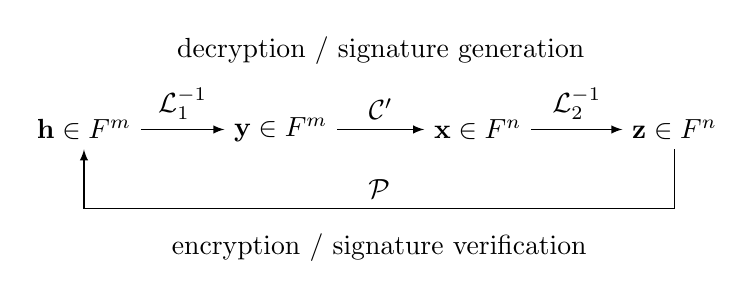
\begin{tikzpicture}
        \node (h) at (-2.5, 0) {$\textbf{h} \in \mathbb{F}^{m}$};
        \node (x) at (0, 0) {$\textbf{y} \in \mathbb{F}^{m}$};
        \node (y) at (2.5, 0) {$\textbf{x} \in \mathbb{F}^{n}$};
        \node (z) at (5, 0) {$\textbf{z} \in \mathbb{F}^{n}$};
        \draw[-latex] (h) -- (x) node[midway,above] {$\mathcal{L}_{1}^{-1}$};
        \draw[-latex] (x) -- (y) node[midway,above] {$\mathcal{C}'$}
          node[midway,yshift=1cm] {decryption / signature generation};
        \draw[-latex] (y) -- (z) node[midway,above] {$\mathcal{L}_{2}^{-1}$};
        \draw[-latex] (z) -- (5, -1) -- (-2.5, -1) node[midway,above]
          {$\mathcal{P}$} node[midway,yshift=-.5cm] {encryption / signature
          verification} -- (h);
      \end{tikzpicture}
    \end{figure}
    \item When $m \leq n$, resulting signature schemes have small signatures
        and large keys
  \end{itemize}
\end{frame}

\begin{frame}
  \frametitle{Rainbow signature scheme}
  \framesubtitle{Overview}
  \begin{itemize}
    \item Created by~\cite{Ding:200506}, currently a finalist of
        the NIST standardization process
    \item Easy description, good balance between signature and key sizes
    \begin{itemize}
      \item Generalized version of Unbalanced Oil and
          Vinegar due to~\cite{Kipnis:199904}
    \end{itemize}
    \item Keys are systems of equations, orders of magnitude larger than
        conventional ones
    \begin{itemize}
      \item RSA at 3072 bits, elliptic curves at 256 bits, Rainbow at roughly
          1 Mb
    \end{itemize}
  \end{itemize}
\end{frame}

\begin{frame}
  \frametitle{Rainbow signature scheme}
  \framesubtitle{Preliminaries}
  \begin{itemize}
    \item Parameters are the order $q$ of a finite field, $u, n \in \mathbb{N}$
        and $0 < v_{1} < \cdots < v_{u} < v_{u + 1} = n$
    \item For $1 \leq \ell \leq u$, set vinegar variables
        $V_{\ell} = \{1, \dots, v_{\ell}\}$ and oil variables
        $O_{\ell} = \{v_{\ell} + 1, \dots, v_{\ell + 1}\}$, with
        $o_{\ell} = |O_{\ell}|$
    \item Consider vector spaces spanned by quadratic Oil-Vinegar polynomials
    \begin{align*}
      P_{\ell} = \sum_{i, j \in V_{\ell}} \alpha_{ij}  x_{i}  x_{j}
        + \sum_{i \in V_{\ell}, j \in O_{\ell}} \beta_{ij}  x_{i}  x_{j}
        + \sum_{i \in V_{\ell} \cup O_{\ell}} \gamma_{i}  x_{i} + \;\; \delta,
        \\ \alpha_{ij}, \beta_{ij}, \gamma_{i}, \delta \in \mathbb{F}_{q}
    \end{align*}
  \end{itemize}
\end{frame}

\begin{frame}
  \frametitle{Rainbow signature scheme}
  \framesubtitle{Key generation}
  \begin{itemize}
    \item Let $m = n - v_{1}$ be the number of equations in the keys
    \item Randomly pick two invertible affine transformations
        $\mathcal{L}_{1} : \mathbb{F}_{q}^{m} \to \mathbb{F}_{q}^{m}$ and
        $\mathcal{L}_{2} : \mathbb{F}_{q}^{n} \to \mathbb{F}_{q}^{n}$
    \item Central map is a function
        $\mathcal{C} : \mathbb{F}_{q}^{n} \to \mathbb{F}_{q}^{m}$
    \begin{itemize}
      \item Exactly $o_{\ell}$ polynomials and their respective coefficients
          are randomly chosen from each $P_{\ell}$
    \end{itemize}
    \item Private key is the triple
        $(\mathcal{L}_{1}, \mathcal{C}, \mathcal{L}_{2})$, public key is the
        composition
        $\mathcal{P} = \mathcal{L}_{1} \circ \mathcal{C} \circ \mathcal{L}_{2}$
     \begin{itemize}
       \item \cite{Wolf:200511} shows that $\mathcal{L}_{1}$ is unneeded if
           $u = 1$
     \end{itemize}
  \end{itemize}
\end{frame}

\begin{frame}
  \frametitle{Rainbow signature scheme}
  \framesubtitle{Preimage of the central map}
  \begin{itemize}
    \item Vinegar variables of a layer are exactly the oil and vinegar
        variables from the previous layer
    \item This enables the inversion of each Oil-Vinegar layer recursively
    \item With $u = 2$, the initial configuration of $\mathcal{C}$ is
    \vspace{.25cm}
    \begin{figure}
      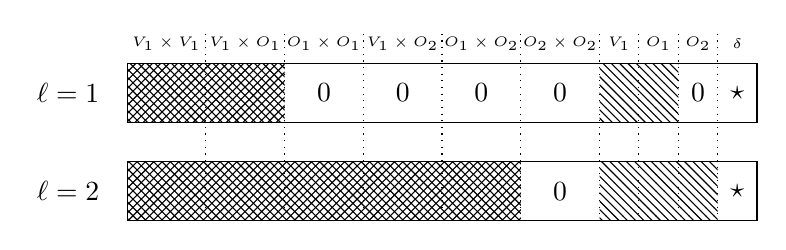
\begin{tikzpicture}
        \node (v1v1) at (0.5, 1) {\tiny $V_{1} \times V_{1}$};
        \node (v1o1) at (1.5, 1) {\tiny $V_{1} \times O_{1}$};
        \node (o1o1) at (2.5, 1) {\tiny $O_{1} \times O_{1}$};
        \node (v1o2) at (3.5, 1) {\tiny $V_{1} \times O_{2}$};
        \node (o1o2) at (4.5, 1) {\tiny $O_{1} \times O_{2}$};
        \node (o2o2) at (5.5, 1) {\tiny $O_{2} \times O_{2}$};
        \node (v1)   at (6.25, 1) {\tiny $V_{1}$};
        \node (o1)   at (6.75, 1) {\tiny $O_{1}$};
        \node (o2)   at (7.25, 1) {\tiny $O_{2}$};
        \node (l)    at (7.75, 1) {\tiny $\delta$};
        \foreach \r in {1, ..., 6, 6.5, 7, 7.5}
          \draw[dotted] (\r, 1.125) to (\r, -1.25);

        \draw (0, 0) rectangle (8, 0.75);
        \node (l1)   at (-0.75, 0.375) {$\ell = 1$};
        \fill[pattern=crosshatch] (0, 0) rectangle (2, 0.75);
        \fill[pattern=north west lines] (6, 0) rectangle (7, 0.75);
        \foreach \r in {2.5, ..., 5.5}
          \node at (\r, 0.375) {$0$};

        \node (o2c1)  at (7.25, 0.375) {$0$};
        \node (lc1)  at (7.75, 0.375) {$\star$};
        \draw (0, -0.5) rectangle (8, -1.25);
        \node (l1)   at (-0.75, -0.875) {$\ell = 2$};
        \fill[pattern=crosshatch] (0, -0.5) rectangle (5, -1.25);
        \fill[pattern=north west lines] (6, -0.5) rectangle (7.5, -1.25);
        \node (o2c2) at (5.5, -0.875) {$0$};
        \node (lc2)  at (7.75, -0.875) {$\star$};
      \end{tikzpicture}
    \end{figure}
  \end{itemize}
\end{frame}

\begin{frame}
  \frametitle{Rainbow signature scheme}
  \framesubtitle{Preimage of the central map}
  \begin{itemize}
    \item Randomly choose variables in $V_{1}$ and substitute them
    \vspace{.25cm}
    \begin{figure}
      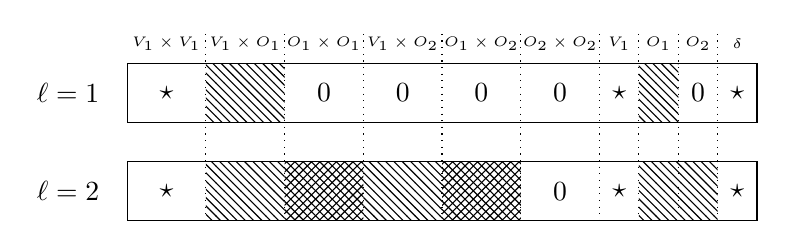
\begin{tikzpicture}
        \node (v1v1) at (0.5, 1) {\tiny $V_{1} \times V_{1}$};
        \node (v1o1) at (1.5, 1) {\tiny $V_{1} \times O_{1}$};
        \node (o1o1) at (2.5, 1) {\tiny $O_{1} \times O_{1}$};
        \node (v1o2) at (3.5, 1) {\tiny $V_{1} \times O_{2}$};
        \node (o1o2) at (4.5, 1) {\tiny $O_{1} \times O_{2}$};
        \node (o2o2) at (5.5, 1) {\tiny $O_{2} \times O_{2}$};
        \node (v1)   at (6.25, 1) {\tiny $V_{1}$};
        \node (o1)   at (6.75, 1) {\tiny $O_{1}$};
        \node (o2)   at (7.25, 1) {\tiny $O_{2}$};
        \node (l)    at (7.75, 1) {\tiny $\delta$};
        \foreach \r in {1, ..., 6, 6.5, 7, 7.5}
          \draw[dotted] (\r, 1.125) to (\r, -1.25);

        \draw (0, 0) rectangle (8, 0.75);
        \node (l1)   at (-0.75, 0.375) {$\ell = 1$};
        \fill[pattern=north west lines] (1, 0) rectangle (2, 0.75);
        \fill[pattern=north west lines] (6.5, 0) rectangle (7, 0.75);
        \foreach \r in {2.5, ..., 5.5, 7.25}
          \node at (\r, 0.375) {$0$};

        \foreach \r in {0.5, 6.25, 7.75}
          \node at (\r, 0.375) {$\star$};

        \draw (0, -0.5) rectangle (8, -1.25);
        \node (l1)   at (-0.75, -0.875) {$\ell = 2$};
        \fill[pattern=north west lines] (1, -0.5) rectangle (2, -1.25);
        \fill[pattern=crosshatch] (2, -0.5) rectangle (3, -1.25);
        \fill[pattern=north west lines] (3, -0.5) rectangle (4, -1.25);
        \fill[pattern=crosshatch] (4, -0.5) rectangle (5, -1.25);
        \fill[pattern=north west lines] (6.5, -0.5) rectangle (7.5, -1.25);
        \foreach \r in {0.5, 6.25, 7.75}
          \node at (\r, -0.875) {$\star$};

        \node at (5.5, -0.875) {$0$};
      \end{tikzpicture}
    \end{figure}
    \item Solve $o_{1}$ linear equations in the first layer to obtain $V_{2}$
        (if possible), and then solve the remaining $o_{2}$ equations
    \vspace{.25cm}
    \begin{figure}
      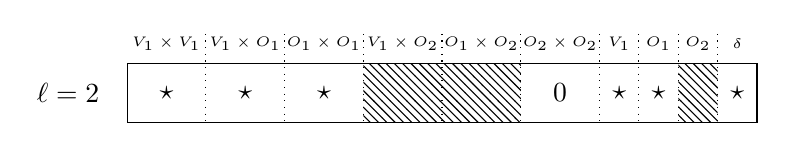
\begin{tikzpicture}
        \node (v1v1) at (0.5, 1) {\tiny $V_{1} \times V_{1}$};
        \node (v1o1) at (1.5, 1) {\tiny $V_{1} \times O_{1}$};
        \node (o1o1) at (2.5, 1) {\tiny $O_{1} \times O_{1}$};
        \node (v1o2) at (3.5, 1) {\tiny $V_{1} \times O_{2}$};
        \node (o1o2) at (4.5, 1) {\tiny $O_{1} \times O_{2}$};
        \node (o2o2) at (5.5, 1) {\tiny $O_{2} \times O_{2}$};
        \node (v1)   at (6.25, 1) {\tiny $V_{1}$};
        \node (o1)   at (6.75, 1) {\tiny $O_{1}$};
        \node (o2)   at (7.25, 1) {\tiny $O_{2}$};
        \node (l)    at (7.75, 1) {\tiny $\delta$};
        \foreach \r in {1, ..., 6, 6.5, 7, 7.5}
          \draw[dotted] (\r, 1.125) to (\r, 0);

        \draw (0, 0) rectangle (8, 0.75);
        \node (l2)   at (-0.75, 0.375) {$\ell = 2$};
        \fill[pattern=north west lines] (3, 0) rectangle (5, 0.75);
        \fill[pattern=north west lines] (7, 0) rectangle (7.5, 0.75);
        \foreach \r in {0.5, ..., 2.5, 6.25, 6.75, 7.75}
          \node at (\r, 0.375) {$\star$};

        \node at (5.5, 0.375) {$0$};
      \end{tikzpicture}
    \end{figure}
  \end{itemize}
\end{frame}

\begin{frame}
  \frametitle{Rainbow signature scheme}
  \framesubtitle{Signature generation}
  \begin{itemize}
    \item Consider a cryptographic hash function $\mathcal{H}$, a message
        $M$, and compute the digest $\textbf{h} = \mathcal{H}(M)$
    \item With possession of the private key, obtain the value
        $\textbf{y} = \mathcal{L}_{1}^{-1}(\textbf{h})$
    \item Generate the preimage of $\textbf{y}$ under the central map,
        $\mathcal{C}(\textbf{x}) = \textbf{y}$, as per the previous operations
    \item Compute the final signature
        $\textbf{z} = \mathcal{L}_{2}^{-1}(\textbf{x})$
  \end{itemize}
\end{frame}

\begin{frame}
  \frametitle{Rainbow signature scheme}
  \framesubtitle{Signature verification}
  \begin{itemize}
    \item Obtain $\textbf{h}$ from the message $M$
    \item With possession of the public key, compute
        $\textbf{h'} = \mathcal{P}(\textbf{z})$
    \item The signature is valid if $\textbf{h} = \textbf{h'}$, and invalid
        otherwise
  \end{itemize}
\end{frame}

\begin{frame}
  \frametitle{Evolution of our research}
  \begin{itemize}
    \item Reduction of key sizes in Rainbow-like schemes
    \begin{itemize}[itemsep=1pt]
      \item Current methods to reduce keys are not usually compatible between
          themselves
      \item To the best of our knowledge, adding structure to the key space is
          a delicate matter
    \end{itemize}
    \item Analysis of choice of vinegar variables in the signature generation
        of Rainbow
    \begin{itemize}[itemsep=1pt]
      \item Early substitution of vinegars in the private key to allow its
          reduction
      \item Consequences of manipulating the randomness of signatures
    \end{itemize}
  \end{itemize}
\end{frame}

\begin{frame}
  \frametitle{Initial proposal}
  \framesubtitle{Approach}
  \begin{itemize}
    \item Recall that vinegar variables are chosen randomly every time
        a preimage of $\mathcal{C}$ is computed
    \item We propose to store $\mathcal{C}$ such that variables in $V_{1}$ are
        already chosen and substituted
    \begin{itemize}
      \item General framework for Rainbow-like schemes, denoted Rainbow-$\eta$
    \end{itemize}
    \item {\small \bibentry{Zambonin:201907}}
  \end{itemize}
\end{frame}

\begin{frame}
  \frametitle{Initial proposal}
  \framesubtitle{Ensuring a preimage of $\mathcal{C}$}
  \begin{itemize}
    \item It may occur that the initial choice of $V_{1}$ leads to unsolvable
        systems of equations in the preimage step
    \begin{itemize}
      \item Low probability for common values of $q$
    \end{itemize}
    \item Maintain the ability for the scheme to correctly sign any message
    \item To obtain the original $\mathcal{C}$, we use a seed or the linear
        relations due to~\cite{Petzoldt:201012}
    \item EU-CMA variant submitted to NIST by~\cite{Ding:201901} makes
        use of a salt that can be modified instead of $V_{1}$
  \end{itemize}
\end{frame}

\begin{frame}
  \frametitle{Initial proposal}
  \framesubtitle{Effect of the construction}
  \begin{itemize}
    \item Preimages with fixed elements are shuffled by $\mathcal{L}_{2}$,
        preserving the randomness of signatures
    \begin{itemize}
      \item Statistical argument through differences of means, std.
          deviations, comparison of CDF and Q-Q plots
    \end{itemize}
    \item Structure of the scheme is unchanged, conventional parameters are
        used
    \begin{itemize}[itemsep=1pt]
      \item To the best of our knowledge, current algebraic cryptanalysis is
          ineffective
      \item Side-channel attacks are not investigated, but we acknowledge that
          regenerating $\mathcal{C}$ is highly detectable
    \end{itemize}
  \end{itemize}
\end{frame}

\begin{frame}
  \frametitle{Initial proposal}
  \framesubtitle{Key pair reductions for newest NIST
    parameters due to~\cite{Ding:202006}}
  \begin{table}[htbp]
    \renewcommand{\arraystretch}{1.2}
    \centering
    \footnotesize
    \begin{tabular}{*{2}{l}*{4}{r}}
      \toprule
      Parameters & Variant & $\#\textbf{sk}$ & $\#\textbf{sk}^{\eta}$
        & $\#\textbf{pk}$ & Difference \\ \midrule
      \multirow{2}{*}{\scriptsize{$(\mathbb{F}_{ 16}, 36, 32, 32)$}}
        & Classic & \multirow{2}{*}{\num{ 103616}}
        & \multirow{2}{*}{\num{  27026}} & \num{  161600} & $-28.88\%$ \\
      & nCyclic & & & \num{   60160} & $-67.13\%$ \\
      \multirow{2}{*}{\scriptsize{$(\mathbb{F}_{256}, 68, 32, 48)$}}
        & Classic & \multirow{2}{*}{\num{ 626016}}
        & \multirow{2}{*}{\num{ 107652}} & \num{  882080} & $-34.37\%$ \\
      & nCyclic & & & \num{  264576} & $-75.32\%$ \\
      \multirow{2}{*}{\scriptsize{$(\mathbb{F}_{256}, 96, 36, 64)$}}
        & Classic & \multirow{2}{*}{\num{1408704}}
        & \multirow{2}{*}{\num{ 204384}} & \num{ 1930600} & $-36.07\%$ \\
      & nCyclic & & & \num{  536104} & $-77.83\%$ \\
      \bottomrule
    \end{tabular}
  \end{table}
\end{frame}

\begin{frame}
  \frametitle{Cryptanalysis of vinegar variables}
  \framesubtitle{Introduction}
  \begin{itemize}
    \item Found in works related only to side-channel attacks
    \begin{itemize}
      \item Introduction of faults leading to zero out or reuse of vinegar
          variables
    \end{itemize}
    \item Practical fault attacks are not easily performed, as argued
        by~\cite{Mus:202011}
    \begin{itemize}
      \item If a user fixes $V_{1}$ through Rainbow-$\eta$, then faults are not
          needed
    \end{itemize}
    \item We propose an attack that leads to an equivalent
        private key from signatures with the same $V_{1}$
    \begin{itemize}
      \item Closely related to the UOV attack due to~\cite{Kipnis:199904}
          that broke balanced OV
    \end{itemize}
  \end{itemize}
\end{frame}

\begin{frame}
  \frametitle{Cryptanalysis of vinegar variables}
  \framesubtitle{Equivalent keys}
  \begin{itemize}
    \item Due to the bipolar construction, there exist equivalent private keys
        that compose to the same public key
    \begin{itemize}
      \item Extended isomorphism of polynomials problem in the case of Rainbow
    \end{itemize}
    \item It is shown by~\cite{Wolf:200511} that there are several redundant
        private keys in the key space of Rainbow
    \begin{itemize}
      \item Security is not reduced if simpler $\mathcal{L}_{1}$ and
          $\mathcal{L}_{2}$ are chosen
    \end{itemize}
    \item Several algebraic attacks are based on finding equivalent keys from
        some structure introduced to the scheme
  \end{itemize}
\end{frame}


\begin{frame}
  \frametitle{Cryptanalysis of vinegar variables}
  \framesubtitle{UOV attack ($u = 1$)}
  \begin{itemize}
    \item The set $\{ (0, \dots, 0, x_{v + 1}, \dots, x_{n}) \in
        \mathbb{F}^{n} \}$ with usual binary operations is the oil subspace
          $\mathcal{O}$, and $\widetilde{\mathcal{O}}
          = \mathcal{L}_{2}^{-1}(\mathcal{O})$
    \item For $f^{(i)}, f^{(j)} \in \mathcal{C}$,
        $f^{(i)} \circ (f^{(j)})^{-1}$ preserves a part of $\mathcal{O}$
          {\tiny (composition of maps from unique symmetric matrices
          out of homogeneous quadratic $f^{(i)}, f^{(j)})$}
    \begin{itemize}[itemsep=1pt]
      \item Similarly, $\widetilde{\mathcal{O}}$ is invariant under
          combinations of public polynomials
    \end{itemize}
    \item Finding the common invariant subspace $\widetilde{\mathcal{O}}$
        leads to an equivalent map $\widetilde{\mathcal{L}}_{2}$, and
          $\textbf{sk'} = (\mathcal{P} \circ \widetilde{\mathcal{L}}_{2},
          \widetilde{\mathcal{L}}_{2}^{-1})$
    \begin{itemize}
      \item Complexity is $q^{n - 1 - 2 \cdot o_{u}} \cdot o_{u}^{4}$ field
          multiplications
    \end{itemize}
  \end{itemize}
\end{frame}

\begin{frame}
  \frametitle{Cryptanalysis of vinegar variables}
  \framesubtitle{Breaking Rainbow-$\eta$}
  \begin{itemize}
    \item UOV attack is also applicable to Rainbow, since it can be interpreted
        as a large, single UOV scheme
    \item If $u = 1$, for any two $\textbf{z}^{(i)}, \textbf{z}^{(j)}$ produced
        with Rainbow-$\eta$, then
          $\mathcal{L}_{2}(\textbf{z}^{(i)} - \textbf{z}^{(j)})
             = (0, \dots, 0, \ast, \dots, \ast) \in \mathcal{O}$
    \item From at least $m + 1$ signatures, obtain $m$ linearly independent
        vectors of $\widetilde{\mathcal{O}}$
    \begin{itemize}
      \item Obtain a basis of the subspace and thus
          $\widetilde{\mathcal{L}}_{2}$
    \end{itemize}
    \item If $u > 1$, we need to solve for the remaining
        $x_{v_{1} + 1}, \dots, x_{v_{u}}$
    \begin{itemize}
      \item Polynomial system with $m$ quadratic equations and $m - o_{u}$
          variables
    \end{itemize}
  \end{itemize}
\end{frame}

\begin{frame}
  \frametitle{Conclusion}
  \begin{itemize}
    \item Elimination of randomness from Rainbow signatures is not recommended
    \begin{itemize}[itemsep=1pt]
      \item Signatures look statistically random but still leak information
      \item Private key size is greatly reduced at the expense of security
    \end{itemize}
    \item Attack in polynomial time if $u = 1$ and all vinegar variables fixed
    \begin{itemize}[itemsep=1pt]
      \item If $u > 1$, performing the attack is easier than all other known
          cryptanalytic methods by a large margin
      \item If $V_{1}$ is only partially fixed, \cite{Shim:202002} argue that
          the resulting scheme is still insecure
    \end{itemize}
  \end{itemize}
\end{frame}

\begin{frame}
  \frametitle{Conclusion}
  \framesubtitle{Open problems}
  \begin{itemize}
    \item Storage of previously used vinegar variables to prevent reuse
    \begin{itemize}
      \item Private key becomes stateful and larger
    \end{itemize}
    \item Poor random number generation on signature generation may be
        exploited
    \item Countermeasures against tampering of intermediate signing steps
    \begin{itemize}[itemsep=1pt]
      \item Checksum alongside signature
      \item Obtain vinegar variables deterministically from private key and
          message
    \end{itemize}
  \end{itemize}
\end{frame}

\backupbegin{}
\begin{frame}[plain, allowframebreaks]
  \frametitle{References}
  \bibliographystyle{apalike}
  {\scriptsize \bibliography{\jobname}}
\end{frame}
\backupend{}

\end{document}
